\documentclass[a4paper,11pt]{article}

\usepackage[T1]{fontenc}
\usepackage[polish]{babel}
\usepackage[utf8]{inputenc}
\usepackage{lmodern}
\selectlanguage{polish}
\usepackage[top=2cm, bottom=2cm, left=3cm, right=3cm]{geometry}
\makeatletter
\newcommand{\linia}{\rule{\linewidth}{0.4mm}}
\renewcommand{\maketitle}{\begin{titlepage}
    \vspace*{2cm}
    \begin{center}\LARGE
    Politechnika Warszawska\\
    Wydział Elektryczny\\
    \end{center}
    \vspace{5cm}
    \noindent\linia
    \begin{center}
      \LARGE \textsc{\@title}
         \end{center}
     \linia
    \vspace{0.5cm}
    \begin{flushright}
    \begin{minipage}{5cm}
    \textit{Autor:}\\
    \normalsize \textsc{\@author} \par
    \end{minipage}
    \vspace{5cm}
     \end{flushright}
    \vspace*{\stretch{6}}
    \begin{center}
    \@date
    \end{center}
  \end{titlepage}%
}
\makeatother
\author{Grzegorz Kopyt}
\title{Specyfikacja Funkcjonalna \\
,,Arbitrage''}
\usepackage{graphicx}

\begin{document}

\maketitle

\tableofcontents
\vspace{1cm}
\noindent\linia
\section{Wstęp teoretyczny}


\noindent\linia
\section{Wymagania funkcjonalne}
\begin{itemize}
\item 
\item 
\item 
\item 
\end{itemize}

\noindent\linia
\section{Obsługa}
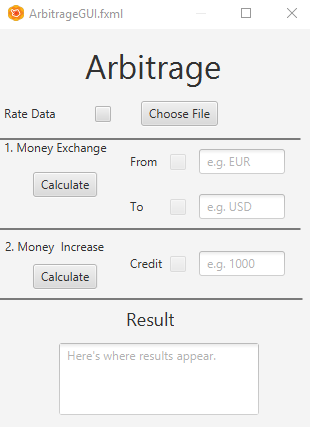
\includegraphics[width=10cm]{ArbitrageGUI}

\begin{itemize}
\item 

\end{itemize}

\noindent\linia
\section{Komunikaty o błędach}
\begin{itemize}
\item 
\end{itemize}

\noindent\linia
\section{Testy akceptacyjne}

\begin{itemize}
\item 

\end{itemize}

\noindent\linia

\end{document}



